\documentclass{article}

% arxiv style (https://github.com/kourgeorge/arxiv-style)
\usepackage{arxiv}

\usepackage[utf8]{inputenc} % allow utf-8 input
\usepackage[T1]{fontenc}    % use 8-bit T1 fonts
\usepackage{natbib}         % citation styles (citet/citep)
\usepackage{hyperref}       % hyperlinks
\usepackage{url}            % simple URL typesetting
\usepackage{booktabs}       % professional-quality tables
\usepackage{amsfonts}       % blackboard math symbols
\usepackage{nicefrac}       % compact symbols for 1/2, etc.
\usepackage{microtype}      % microtypography
\usepackage{xcolor}         % colors
\usepackage{upquote}
\usepackage{fancyvrb}
\usepackage{float}
\usepackage{xspace}      % smart spacing after macros


\usepackage{soul}
\definecolor{deepblue}{rgb}{0,0,0.5}
\definecolor{deepred}{rgb}{0.6,0,0}
\definecolor{deepgreen}{rgb}{0,0.5,0}

\usepackage{listings}
\usepackage{graphicx}
\usepackage{courier}
% \usepackage{color}


% Improved lstListing settings based on https://gist.github.com/mpdehnel/cc43e89a09c18ef6a602
\definecolor{mygreen}{rgb}{0,0.6,0}
\definecolor{mygray}{rgb}{0.5,0.5,0.5}
\definecolor{mymauve}{rgb}{0.58,0,0.82}
\lstset{ %
  backgroundcolor=\color{white},   % choose the background color; you must add \usepackage{color} or \usepackage{xcolor}
  basicstyle=\footnotesize\ttfamily,        % the size of the fonts that are used for the code
  breakatwhitespace=false,         % sets if automatic breaks should only happen at whitespace
  breaklines=false,                 % sets automatic line breaking
  captionpos=none,                    % sets the caption-position to bottom
  commentstyle=\color{gray},    % comment style
  deletekeywords={...},            % if you want to delete keywords from the given language
  escapeinside={\%*}{*)},          % if you want to add LaTeX within your code
  extendedchars=true,              % lets you use non-ASCII characters; for 8-bits encodings only, does not work with UTF-8
  frame=single,                    % adds a frame around the code
  keepspaces=true,                 % keeps spaces in text, useful for keeping indentation of code (possibly needs columns=flexible)
  keywordstyle=\color{blue},       % keyword style
  language=Python,                 % the language of the code
  otherkeywords={*,...},            % if you want to add more keywords to the set
  numbers=left,                    % where to put the line-numbers; possible values are (none, left, right)
  numbersep=5pt,                   % how far the line-numbers are from the code
  numberstyle=\tiny\color{mygray}, % the style that is used for the line-numbers
  rulecolor=\color{black},         % if not set, the frame-color may be changed on line-breaks within not-black text (e.g. comments (green here))
  showspaces=false,                % show spaces everywhere adding particular underscores; it overrides 'showstringspaces'
  showstringspaces=false,          % underline spaces within strings only
  showtabs=false,                  % show tabs within strings adding particular underscores
  stepnumber=2,                    % the step between two line-numbers. If it's 1, each line will be numbered
  stringstyle=\color{mymauve},     % string literal style
  tabsize=2,                       % sets default tabsize to 2 spaces
  numbers=none,
  title=\lstname                   % show the filename of files included with \lstinputlisting; also try caption instead of title
}


\DeclareFixedFont{\ttb}{T1}{txtt}{bx}{n}{10} % for bold
\DeclareFixedFont{\ttm}{T1}{txtt}{m}{n}{10}  % for normal

\DeclareFixedFont{\ttbsmall}{T1}{txtt}{bx}{n}{8} % for bold
\DeclareFixedFont{\ttmsmall}{T1}{txtt}{m}{n}{8}  % for normal

% Python style for highlighting
\newcommand\pythonstyle{\lstset{
language=Python,
basicstyle=\ttm,
morekeywords={self},              % Add keywords here
keywordstyle=\ttb\color{deepblue},
emph={MyClass,__init__},          % Custom highlighting
emphstyle=\ttb\color{deepred},    % Custom highlighting style
stringstyle=\color{deepgreen},
frame=tb,                         % Any extra options here
showstringspaces=false
}}


% Python environment
\lstnewenvironment{python}[1][]
{
\pythonstyle
\lstset{#1}
}
{}

% Python for external files
\newcommand\pythonexternal[2][]{{
\pythonstyle
\lstinputlisting[#1]{#2}}}

% Python for inline
\newcommand\pythoninline[1]{{\pythonstyle\lstinline!#1!}}

% Python small style for highlighting
\newcommand\pythonsmallstyle{\lstset{
language=Python,
basicstyle=\ttmsmall,
morekeywords={self},              % Add keywords here
keywordstyle=\ttbsmall\color{deepblue},
emph={MyClass,__init__},          % Custom highlighting
emphstyle=\ttbsmall\color{deepred},    % Custom highlighting style
stringstyle=\color{deepgreen},
frame=tb,                         % Any extra options here
showstringspaces=false
}}


% Python environment
\lstnewenvironment{pythonsmall}[1][]
{
\pythonsmallstyle
\lstset{#1}
}
{}


% Bash style for highlighting
\newcommand\bashstyle{\lstset{
language=bash,
basicstyle=\ttm,
morekeywords={},              % Add keywords here
keywordstyle=\ttm,%\ttb\color{deepblue},
emph={},          % Custom highlighting
emphstyle=\ttb\color{deepred},    % Custom highlighting style
stringstyle=\color{deepgreen},
frame=tb,                         % Any extra options here
showstringspaces=false
}}


% Python environment
\lstnewenvironment{bash}[1][]
{
\bashstyle
\lstset{#1}
}
{}

% Python for external files
\newcommand\bashexternal[2][]{{
\bashstyle
\lstinputlisting[#1]{#2}}}

% Python for inline
\newcommand\bashinline[1]{{\bashstyle\lstinline!#1!}}

\newcommand{\todoAD}[1]{\color{red} [\textbf{AD: } #1]}

% Single source of truth for collection-level statistics. Update these in one
% place so the abstract, introduction, and conclusion stay consistent.
\newcommand{\numdatasets}{338\xspace}
\newcommand{\numtrajectories}{350K\xspace}
\newcommand{\numsteps}{55M\xspace}
\newcommand{\datasetsize}{56\,GB\xspace}


%\title{Minari: Facilitating Community-Based Reinforcement Learning Datasets}
\title{Minari: Infrastructure for Collaborative Reinforcement Learning Datasets}

% Uncomment to override the `A preprint' in the header
%\renewcommand{\headeright}{Technical Report}
%\renewcommand{\undertitle}{Technical Report}
\renewcommand{\shorttitle}{Minari}

% The \author macro works with any number of authors. There are two commands
% used to separate the names and addresses of multiple authors: \And and \AND.
%
% Using \And between authors leaves it to LaTeX to determine where to break the
% lines. Using \AND forces a line break at that point. So, if LaTeX puts 3 of 4
% authors names on the first line, and the last on the second line, try using
% \AND instead of \And before the third author name.

\author{%
  Omar G.~Younis \\
  Farama Foundation, Mila \\
  \And
  Rodrigo Perez-Vicente \\
  Farama Foundation \\
  \And
  John U.~Balis \\
  Farama Foundation, Mila \\
  \AND
  Alex Davey \\
  Farama Foundation, INRIA \\
  \And
  Will Dudley \\
  Farama Foundation \\
  \And
  Jordan K.~Terry \\
  Farama Foundation \\
}

\begin{document}

\maketitle

\begin{abstract}
Sharing and reusing agent experience is central to advancing reinforcement learning (RL), yet today this remains difficult: datasets are distributed in inconsistent formats, are poorly documented, and are rarely reproducible. We introduce \emph{Minari}, an open-source library that standardizes the collection, sharing, and ingestion of RL trajectories. Inspired by the design principles of Gym and Gymnasium, Minari exposes a familiar and extensible API that supports the entire dataset lifecycle: researchers can collect trajectories from any environment, annotate them with metadata, filter, combine, and shuffle datasets, and publish or download them with a single command through native integration with the HuggingFace Hub. Reproducibility is a first-class concern: Minari preserves environment specifications, seeds, applied wrappers, and software requirements so that datasets can be faithfully reconstructed and regenerated.
Minari is already adopted by major offline RL frameworks, including TorchRL, AgileRL, and d3rlpy, allowing users to swap or merge datasets by changing a single line of code. It ships with a curated collection of \numdatasets reproducible datasets spanning robotic locomotion and manipulation, maze and grid navigation, text-based instruction following, Atari games, hierarchical planning, and web-agent interaction, totaling \numtrajectories trajectories and \numsteps interaction steps. By lowering the barrier to sharing and reusing agent experience, Minari aims to establish a community standard that accelerates collaborative progress in offline RL.
\end{abstract}

% keywords can be removed
\keywords{Reinforcement Learning \and Offline RL \and Datasets \and Benchmarks \and Open Source}

\section{Introduction}

As we enter the \textit{Era of Experience} \cite{experience-era}, where learning from interactions becomes crucial for AI progress, the data generated by intelligent agents represents an increasingly valuable resource. This data encapsulates how agents interact with environments over time and the outcome of these interactions. Despite its growing importance, the sharing and reuse of agent experience remains limited and fragmented.

Three critical challenges impede progress in this domain. First, agent experience data is rarely collected or distributed in standardized formats, creating immediate barriers to interoperability. Second, when experience datasets are shared, they are typically not reproducible, have inconsistent documentation, or environment-specific assumptions that complicate integration and reuse. Third, combining datasets from different sources into a coherent and usable form is particularly challenging, requiring significant manual effort and domain-specific adjustments. This lack of standardization impedes collaboration and slows down progress in the field. 

To address these limitations, we introduce Minari, an open-source library designed to streamline the collection, sharing, and ingestion of agent experience. Minari provides a unified interface for reinforcement learning datasets inspired by the design philosophy of Gym and Gymnasium \cite{gym, gymnasium}, offering a familiar and extensible API for interacting with trajectory data. A simple example usage is given in Figure ~\ref{fig:code}, and is described in detail in Sect.~\ref{sec:library_features}. Our primary objective is to establish a robust standard for reinforcement learning datasets that enhances interoperability, improves reproducibility, and facilitates collaboration across the research community.

Minari supports the full dataset lifecycle: researchers can collect trajectories from any environment, annotate and manipulate them, and upload them to the HuggingFace Hub\footnote{https://huggingface.co} or other cloud platforms with a single command. Datasets can also be downloaded, inspected, and combined via a simple command-line interface or Python API. This enables seamless integration with training libraries and workflows, allowing users to swap or merge datasets by changing a single line of code.

By standardizing experience data and lowering the barrier to sharing and reuse, Minari paves the way for large scale, collaborative progress in reinforcement learning.

\paragraph{Contributions.} In summary, this paper makes the following contributions:
\begin{itemize}
    \item \textbf{A standard and library for RL datasets.} We define a flexible, environment-agnostic format for trajectory data with rich, machine-readable metadata and consistent naming conventions, and implement it in an open-source, pip-installable library with both a Python API and a command-line interface (Sect.~\ref{sec:library_features}).
    \item \textbf{Reproducibility by construction.} Minari records environment specifications, generation seeds, applied wrappers, and pinned software requirements, enabling datasets to be exactly reconstructed and regenerated, an explicit improvement over prior offline RL benchmarks (Sect.~\ref{sec:repro}).
    \item \textbf{A large, curated, and growing dataset collection.} We release \numdatasets reproducible datasets (\numtrajectories trajectories, \numsteps steps) across seven domains, each documented and accompanied by public generation scripts (Sect.~\ref{sec:datasets}).
    \item \textbf{Ecosystem integration.} Minari is natively supported by widely used offline RL libraries (TorchRL, AgileRL, d3rlpy) and built on the HuggingFace Hub, making datasets immediately usable in existing training pipelines.
\end{itemize}

\begin{figure}[t]
    \centering
   \begin{pythonsmall}
  import minari
  import gymnasium as gym
  env = gym.make('CartPole-v1')
  env = minari.DataCollector(env, record_infos=True)
  ... # Step through environment as usual
  dataset = env.create_dataset("cartpole/test-v0")\end{pythonsmall}
   \begin{pythonsmall}
  import minari
  dataset = minari.load_dataset('D4RL/door/human-v2', download=True)
  episodes = dataset.sample_episodes(n_episodes=5) # Sample 5 episodes
  env = dataset.recover_environment() # Optionally recover data collection env\end{pythonsmall}
  \caption{Two examples of Minari usage. \textbf{Top:} Creating a Minari dataset using the Gymnasium wrapper. Non-Gymnasium environments are also supported and can be created manually via \lstinline|minari.create_dataset_from_buffers()|. \textbf{Bottom:} Loading an existing dataset (local or remote). In many cases one can instead directly use one of the integrations with existing Offline RL  libraries described in Sec.~\ref{sec:integrations}.}
    \label{fig:code}
\end{figure}

\section{Related work}
Several open-source libraries inspired and laid the foundation for the development of Minari. Table~\ref{tab:comparison} situates Minari with respect to the most closely related efforts: unlike fixed benchmark releases such as D4RL and RL Unplugged, Minari is a general-purpose library that lets practitioners \emph{create}, \emph{document}, \emph{version}, and \emph{share} their own datasets, while remaining framework-agnostic and reproducible by construction.

\begin{table}[h]
    \centering
    \footnotesize
    \setlength{\tabcolsep}{4pt}
    \resizebox{\textwidth}{!}{%
    \begin{tabular}{@{}lcccccc@{}}
    \toprule
     & \textbf{Standard} & \textbf{User-created} & \textbf{Repro-} & \textbf{Hub} & \textbf{Framework-} & \textbf{Domain} \\
     & \textbf{format} & \textbf{datasets} & \textbf{ducible} & \textbf{sharing} & \textbf{agnostic} & \textbf{scope} \\
    \midrule
    D4RL \cite{d4rl}                 & \checkmark & --         & --         & --         & \checkmark & RL \\
    RL Unplugged \cite{rlunplugged}  & \checkmark & --         & --         & --         & \checkmark & RL \\
    RLDS \cite{rlds}                 & \checkmark & \checkmark & --         & partial    & TF only    & RL \\
    LeRobot \cite{lerobot}           & \checkmark & \checkmark & partial    & \checkmark & PyTorch    & Robotics \\
    \textbf{Minari (ours)}           & \checkmark & \checkmark & \checkmark & \checkmark & \checkmark & General \\
    \bottomrule
    \end{tabular}%
    }
    \caption{Comparison of Minari with related dataset libraries and benchmarks for sequential decision-making. ``Reproducible'' denotes built-in mechanisms to reconstruct the data-generating environment (specs, seeds, wrappers, and software requirements); ``Hub sharing'' denotes one-command publishing/downloading to a community hub.}
    \label{tab:comparison}
\end{table}

\paragraph{RLDS} The Reinforcement Learning Datasets (RLDS) \cite{rlds} provides a framework for storing and manipulating RL trajectories using TensorFlow-based data structures. RLDS introduced a standardized schema for trajectory data and offers efficient operations for data manipulation, from which we take inspiration while developing Minari. However, its tight coupling with the TensorFlow ecosystem limits its accessibility.

\paragraph{D4RL} The Dataset for Data-Driven Deep Reinforcement Learning (D4RL) \cite{d4rl} was one of the first major benchmarks for offline RL, providing a collection of tasks and pre-recorded datasets to evaluate algorithms. While D4RL made significant contributions by establishing baseline performance metrics across various domains, its datasets are tied to specific environment versions and cannot be reliably reproduced. Additionally, D4RL does not offer tools for practitioners to create and share their datasets. Minari addresses these limitations by providing a comprehensive toolset for dataset creation, manipulation, and distribution while ensuring version compatibility and reproducibility.

\paragraph{RL Unplugged} RL Unplugged \cite{rlunplugged} represents another significant contribution to offline reinforcement learning research, providing a diverse suite of tasks and corresponding datasets across domains including DeepMind Control Suite \cite{deepmindcontrolsuite}, and Atari games. Similar to D4RL, it enables benchmarking of offline RL algorithms but with a stronger emphasis on challenging exploration scenarios. However, it shares D4RL's limitations regarding reproducibility and extensibility, as datasets are provided as fixed collections without standardized tools for researchers to create compatible datasets of their own.

\paragraph{LeRobot} LeRobot \cite{lerobot} is an open-source library that provides models, datasets, and tools for robotics in PyTorch. Although LeRobot provides valuable resources to the robotics community, its focus remains specifically on real-world robotics applications rather than general agent learning. On the other hand, Minari provides a generalized framework designed for all types of intelligent agents.

\paragraph{HuggingFace Hub} The HuggingFace Hub has emerged as a central repository for machine learning models and datasets, particularly in the natural language processing domain. Its infrastructure for version control, documentation, and community collaboration has positively impacted resource sharing in deep learning. While not specifically designed for reinforcement learning data, HuggingFace Hub provides valuable infrastructure for hosting datasets. Minari leverages this infrastructure by implementing native integration with the Hub, enabling researchers to publish, version, and download reinforcement learning datasets.

\subsection{Library integrations}
\label{sec:integrations}
Minari is natively supported by many of the most popular libraries supporting offline RL training, making it easy to use Minari datasets in training pipelines. We list here the libraries that natively integrate Minari.

\paragraph{TorchRL} TorchRL \cite{torchrl} is a PyTorch-based library for reinforcement learning that provides modular and flexible tools to build and train RL agents. It supports a wide range of environments and integrates tightly with the PyTorch ecosystem. The library is designed to be scalable and customizable for both research and production applications.

\paragraph{AgileRL}
AgileRL \cite{agilerl} is an open-source library designed to automate the process of designing and optimizing reinforcement learning agents. It focuses on enabling fast experimentation by using meta-learning and population-based training to evolve agent architectures and hyperparameters. AgileRL is particularly suited for practitioners who want to quickly prototype high-performing agents without deep RL expertise.

\paragraph{D3RLPY}
d3rlpy \cite{d3rlpy} is a data-driven deep reinforcement learning library. It provides implementations of state-of-the-art offline RL algorithms like CQL \cite{CQL}, BCQ \cite{BCQ}, and TD3+BC \cite{TD3+BC} with easy-to-use APIs built on top of PyTorch.


\section{Library features}
\label{sec:library_features}

\subsection{Dataset standards}
Minari establishes a comprehensive standard for reinforcement learning datasets that promotes interoperability and reproducibility. The library adopts a consistent and descriptive naming convention for datasets using the following syntax:
\begin{verbatim}
    namespace/environment/dataset_name-v(version)
\end{verbatim}
where the \verb|namespace| enables logical grouping of related datasets, \verb|environment| indicates the name of the data source environment, \verb|dataset| names describe the content, and version numbers track iterations; only the dataset name is mandatory. For example, a human demonstration dataset from the \textit{AdroitHandDoor} environment would be identified as \verb|door/human-v0|, or if grouped under a namespace like D4RL, as \verb|D4RL/door/human-v0|.

Each dataset is stored with rich metadata that captures essential information about it. The default dataset metadata includes identifiers, the total number of episodes and steps, data source environment specifications (if available), action and observation spaces, code references, authorship information, algorithm details, and version compatibility requirements for full reproducibility. Additionally, episode-level metadata provides statistical summaries of rewards (maximum, minimum, mean, standard deviation, and sum), enabling efficient filtering and selection of episodes for training or evaluation.

The core data encapsulates all information from the agent's interaction with the environment. This is structured as a sequence of episodes, where each episode includes observations, actions, rewards, termination and truncation flags, and optional information dictionaries. The flexible format accommodates various types of actions and observations while maintaining strict consistency in structure, ensuring that datasets can be easily preprocessed and combined. This standardization is particularly valuable for offline reinforcement learning, where algorithms often require consistent data representations across diverse environments and tasks.

Minari supports multiple file formats seamlessly integrated through the Python library's unified API. Specifically, it offers HDF5 formatting for quick plug-and-play with small datasets, as well as Arrow and Parquet formats optimized for large-scale distributed training.

\subsection{Minari software package}
\begin{table}[]
    \centering
    \begin{tabular}{cc}
    \toprule
    \textbf{Command name} & \textbf{Description}\\
    \midrule
     \bashinline{list local} & List Minari datasets in local storage. \\
     \bashinline{list remote} & List Minari datasets in remote storage. \\
     %\hline
     \bashinline{show} & Describe a local or remote dataset, and its environment. \\
     %\hline
     \bashinline{delete} & Delete datasets from local database. \\
     %\hline
     \bashinline{download} & Download Minari datasets from remote server.\\
     %\hline
     \bashinline{upload} & Upload Minari datasets to the specified remote server. \\
     %\hline
     \bashinline{combine} & Combine multiple datasets into a single dataset.\\
     \bottomrule
    \end{tabular}
    \caption{List of available commands in the Minari command line interface, along with their description. To use a command append minari before the command name, e.g. \textit{minari list local}; \textit{-\,-help} can be used for more information.}
    \label{tab:cli}
\end{table}

Minari offers a comprehensive set of features to create, read, manipulate, and share reinforcement learning datasets. The library is designed with a focus on ease of use while maintaining the flexibility needed for diverse research applications. It can be downloaded easily from the Python Package Index (PyPI), making installation straightforward across various platforms and environments.

For convenience, specifically for common one-time operations on datasets such as download or merge, Minari provides a set of commands that are executable directly from the terminal. We provide a complete list of these commands in Table \ref{tab:cli}, enabling researchers to perform essential dataset operations without writing Python code.
To create a new dataset, we provide two primary methods: using a Gymnasium wrapper, which automatically collects the data from the environment during agent interaction (see Fig.~\ref{fig:code}), or by adding data to a buffer object, which can then be serialized to disk in the Minari format. The Gymnasium wrapper approach is particularly useful for recording live agent experiences with minimal code changes, while the buffer approach offers more control over the dataset creation process and enables the integration of data from non-Gymnasium environments or external sources. For image-based environments, Minari optionally applies JPEG encoding to observations, substantially reducing on-disk and download size for pixel datasets such as Atari while preserving the original frames.

The library also provides utilities for dataset manipulation, allowing researchers to filter episodes based on specific criteria, combine datasets from different sources, and efficiently shuffle the data.
Minari's integration with the HuggingFace Hub enables seamless sharing of datasets with the research community. Researchers can publish their datasets with a single command, making their experimental data available for verification and extension. Similarly, published datasets can be downloaded and used in experiments with minimal effort, promoting reproducibility and building upon existing work.

\subsection{Improving reproducibility in Offline RL}
\label{sec:repro}

Reproducibility represents a crucial challenge in reinforcement learning \cite{hendersonDeepReinforcementLearning2019}, particularly in offline RL where dataset variability introduces additional complexity. Discrepancies in the environment, even minor ones, can create a misalignment between data generation and evaluation conditions. Minari addresses these reproducibility challenges through three key design innovations.

First, its \pythoninline{dataset.recover_environment()} utility reconstructs not only the original Gymnasium environment that generated the dataset but also preserves the applied wrappers that modified environmental parameters. Second, Minari automatically preserves generation seeds, even if the user does not explicitly set them, ensuring consistent data recollection. 
Finally, variations in the environment can also be introduced by changes in the underlying software implementation, especially for physics-based environments such as MuJoCo~\cite{mujoco} which use numerical integration to model rigid-body dynamics. To help control this, pip requirements can be specified during the creation of a dataset, and Minari will automatically check to ensure that the current set of installed packages is compatible with the requirement specification.

\section{Available datasets}
\label{sec:datasets}

Minari is distributed with a comprehensive collection of curated datasets, accessible through our HuggingFace repository. The collection currently comprises \numdatasets diverse datasets (\numtrajectories trajectories, \numsteps steps) totaling \datasetsize in our remote repository, and it continues to grow with community contributions. To ensure complete reproducibility, we provide the dataset generation scripts in a public GitHub repository\footnote{https://github.com/Farama-Foundation/minari-dataset-generation-scripts}. Table~\ref{tab:collections} summarizes the collection by domain; the following subsections describe each group in detail. Every dataset is thoroughly documented with specifications and usage guidelines in the official documentation\footnote{https://minari.farama.org}, enabling researchers to easily reproduce and extend our datasets.

\begin{table}[h]
    \centering
    \footnotesize
    \begin{tabular}{@{}lllll@{}}
    \toprule
    \textbf{Collection} & \textbf{Domain} & \textbf{Observations} & \textbf{\# Datasets} & \textbf{Data source} \\
    \midrule
    D4RL      & Locomotion, manipulation, navigation & State / grid & 31  & Planners, RL, human, IL \\
    MuJoCo    & Continuous control                   & State        & 26  & SAC / TQC (SB3) \\
    BabyAI    & Instruction following                & Grid / text  & 170 & Expert bot policy \\
    Atari     & Arcade games                         & Pixels       & 57  & PPO (CleanRL) \\
    MetaWorld & Robotic manipulation                 & State        & 50  & Scripted expert \\
    WebAgents & Web navigation                       & Text         & 4   & Human (WebLINX) \\
    \bottomrule
    \end{tabular}
    \caption{Overview of the dataset collections shipped with Minari. Counts are approximate and grow over time; per-dataset statistics (episodes, steps, returns) are available in the documentation and in each dataset's metadata. Together these collections span discrete and continuous actions and state-, grid-, pixel-, and text-based observations.}
    \label{tab:collections}
\end{table}

\subsection{D4RL}
\begin{figure}[t!]
    \centering
    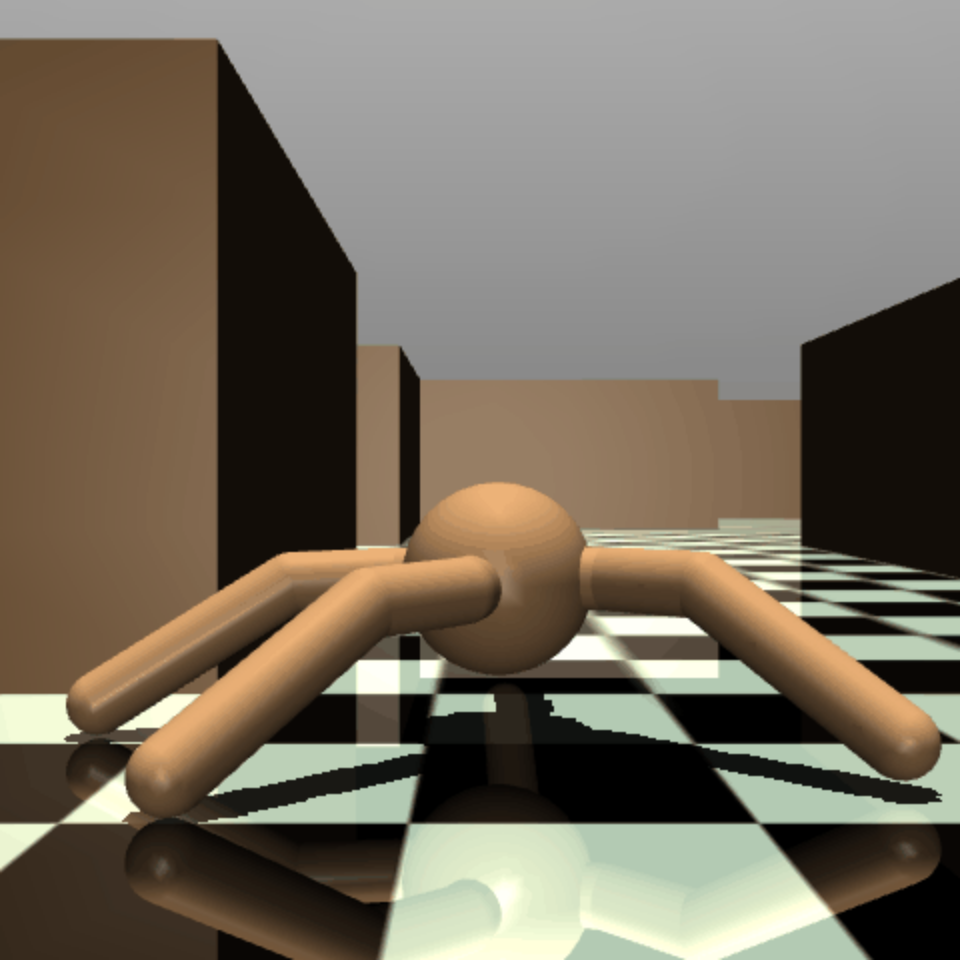
\includegraphics[width=0.18\linewidth]{figs/d4rl_ant.png}
    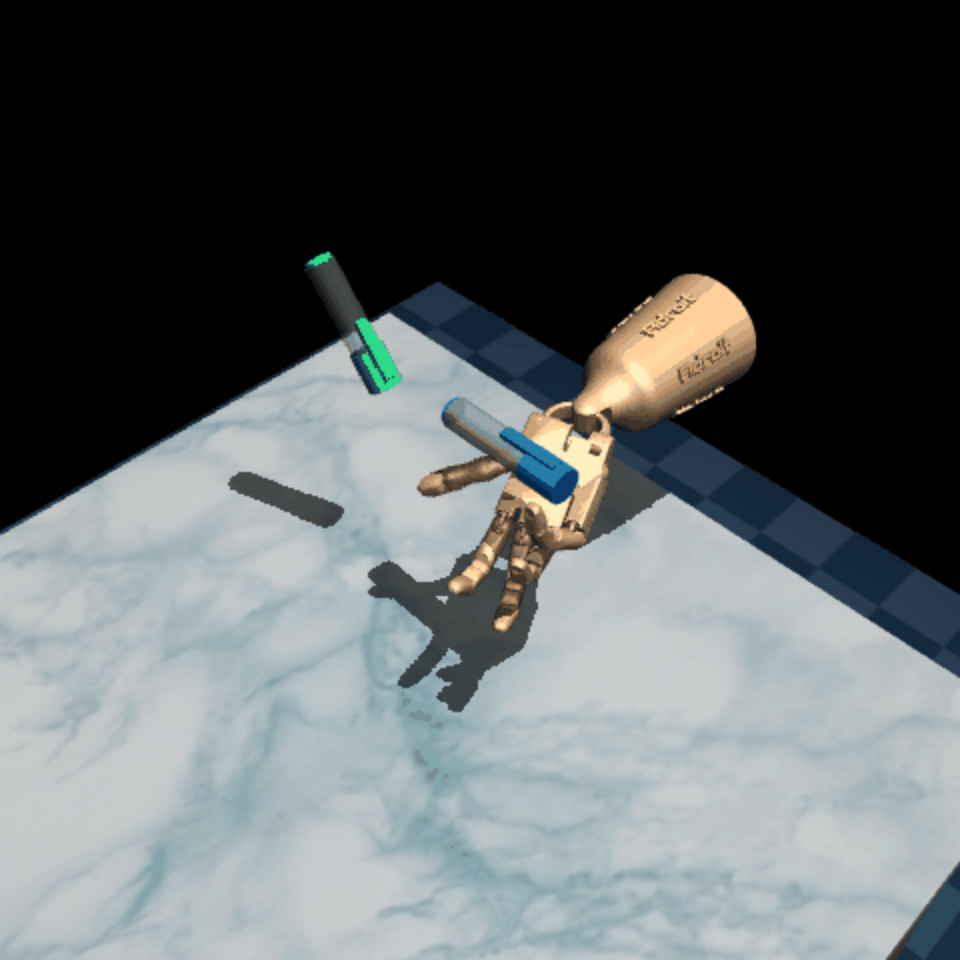
\includegraphics[width=0.18\linewidth]{figs/d4rl_pen.png}
    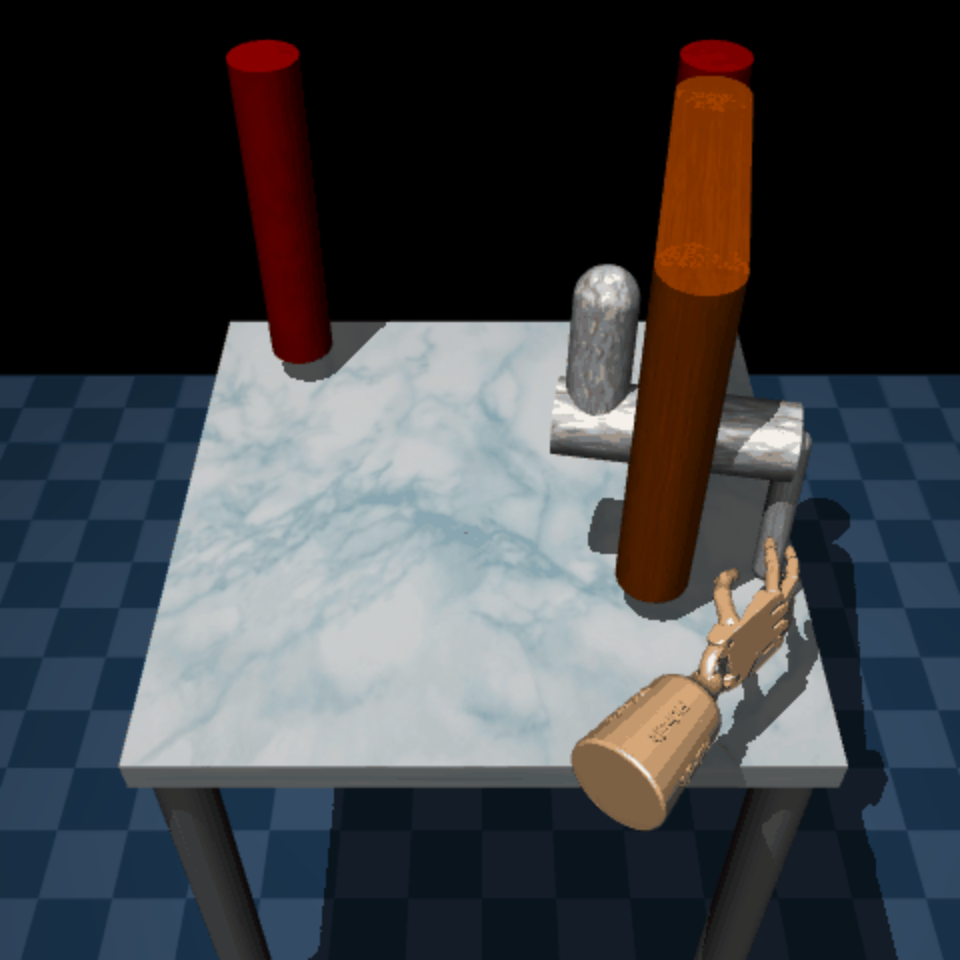
\includegraphics[width=0.18\linewidth]{figs/d4rl_door.png}
    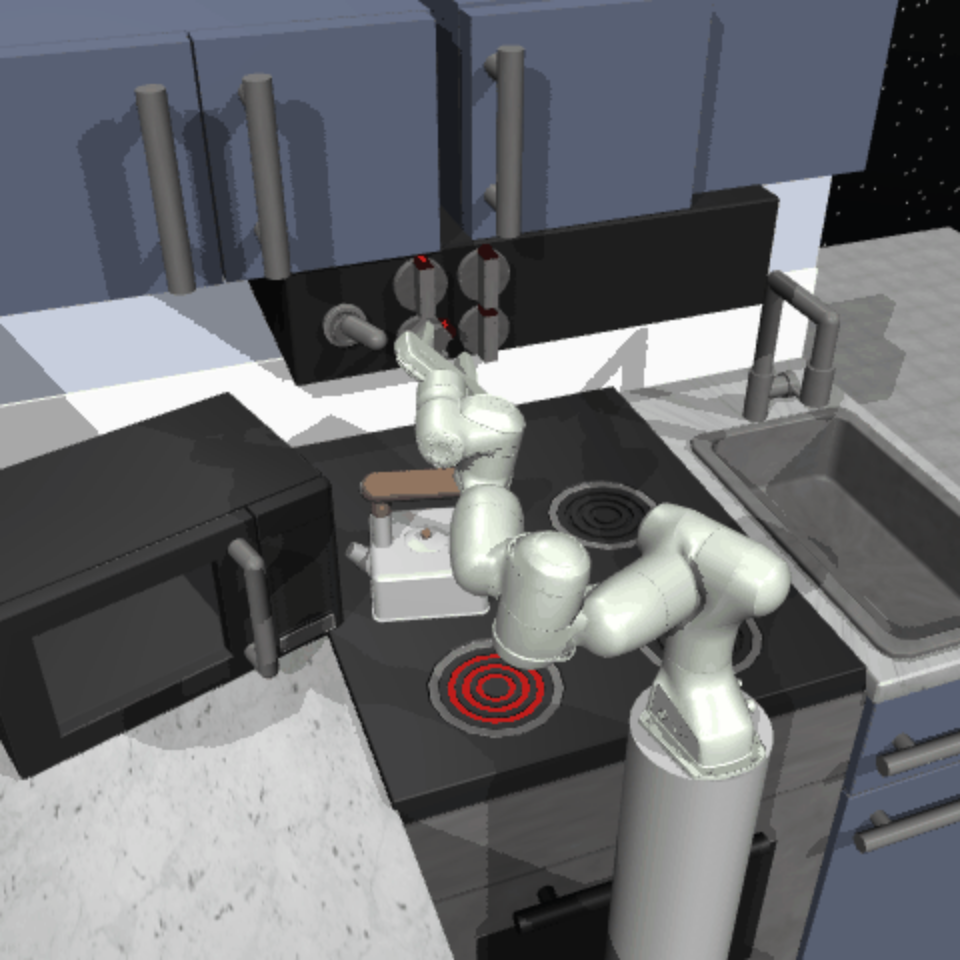
\includegraphics[width=0.18\linewidth]{figs/d4rl_kitchen.png}
    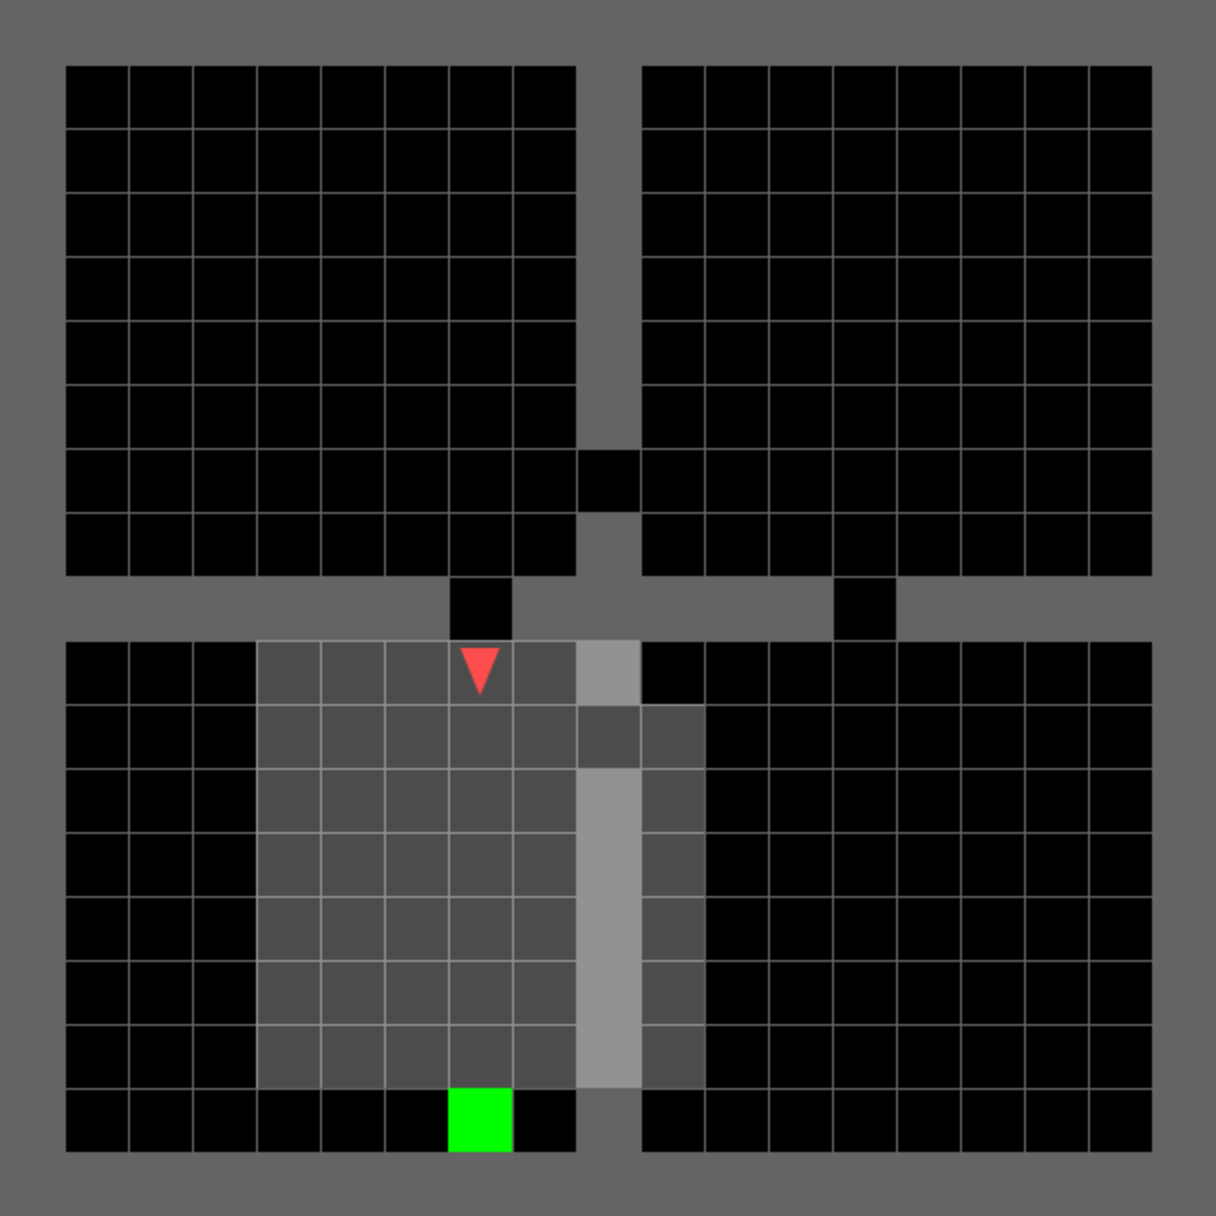
\includegraphics[width=0.18\linewidth]{figs/d4rl_minigrid.png}
    \caption{Representative D4RL environments (left to right): \textsc{Ant Maze}, \textsc{Pen}, \textsc{Door}, \textsc{Kitchen}, and \textsc{Minigrid}. \textsc{Point Maze}, \textsc{Hammer}, and \textsc{Relocate} are also part of the collection (Sec.~\ref{sec:datasets}) but not shown here.}
    \label{fig:dr4l}
\end{figure}
\begin{table}[]
\footnotesize
\centering
\begin{tabular}{@{}lllllll@{}}
\toprule
                             & BC    & BC-10\% & TD3+BC & AWAC  & CQL   & IQL   \\ \midrule
pointmaze/umaze-v2           & 53.8  & 55.1    & 71.9   & 52.3  & 85.5  & 52.4  \\
pointmaze/medium-v2          & 78.8  & 59.3    & 105.8  & 85.3  & 80.7  & 38.6  \\
pointmaze/large-v2           & 42.3  & 36.9    & 80.1   & 111.8 & 63.3  & 43.3  \\ \midrule
\textit{pointmaze average}   & 58.3  & 50.4    & 85.9   & 83.1  & 76.5  & 44.8  \\ \midrule
antmaze/umaze-v2             & 97.7  & 92.0    & 97.7   & 100.0 & 46.3  & 87.7  \\
antmaze/umaze-diverse-v2     & 95.3  & 89.7    & 96.7   & 96.7  & 79.0  & 87.7  \\
antmaze/medium-play-v2       & 36.7  & 34.0    & 59.3   & 70.0  & 33.0  & 41.3  \\
antmaze/medium-diverse-v2    & 16.3  & 11.0    & 23.3   & 56.7  & 5.7   & 21.3  \\
antmaze/large-play-v2        & 20.0  & 22.7    & 32.7   & 86.7  & 20.7  & 29.0  \\
antmaze/large-diverse-v2     & 16.0  & 14.7    & 23.3   & 26.7  & 6.7   & 24.3  \\ \midrule
\textit{antmaze average}     & 47.0  & 44.0    & 55.5   & 72.8  & 31.9  & 48.6  \\ \midrule
pen/human-v2                 & 56.9  & 17.5    & 0.4    & 77.3  & 35.4  & 64.0  \\
pen/cloned-v2                & 68.0  & 42.0    & 36.6   & 77.8  & 14.3  & 79.6  \\
pen/expert-v2                & 110.4 & 62.2    & 114.7  & 118.7 & 18.8  & 117.1 \\ \midrule
\textit{pen average}         & 78.4  & 40.6    & 50.6   & 91.3  & 22.8  & 86.9  \\ \midrule
door/human-v2                & 6.0   & 0.4     & 0.5    & 13.9  & 8.0   & 9.8   \\
door/cloned-v2               & 0.3   & 5.2     & 0.5    & 5.7   & 0.5   & 5.4   \\
door/expert-v2               & 104.3 & 105.2   & 2.8    & 105.1 & 85.7  & 106.1 \\ \midrule
\textit{door average}        & 36.9  & 36.9    & 1.3    & 41.6  & 31.4  & 40.4  \\ \midrule
hammer/human-v2              & 15.4  & 10.4    & 6.6    & 27.6  & 0.3   & 11.6  \\
hammer/cloned-v2             & 14.8  & 17.4    & 2.1    & 6.5   & 0.3   & 27.6  \\
hammer/expert-v2             & 131.5 & 132.9   & 102.5  & 132.6 & 0.3   & 133.4 \\ \midrule
\textit{hammer average}      & 53.9  & 53.6    & 37.1   & 55.6  & 0.3   & 57.5  \\ \midrule
relocate/human-v2            & 1.5   & 0.2     & 0.2    & 1.2   & 0.2   & 0.7   \\
relocate/cloned-v2           & 0.2   & 0.2     & 0.3    & 0.2   & 0.3   & 0.7   \\
relocate/expert-v2           & 106.7 & 98.4    & 1.2    & 107.2 & 0.3   & 106.7 \\ \midrule
\textit{relocate average}    & 36.1  & 32.9    & 0.6    & 36.2  & 0.3   & 36.0  \\ \bottomrule
\end{tabular}
\caption{Normalized scores of offline RL algorithms on the D4RL navigation and manipulation datasets reproduced in Minari, using the CORL~\cite{corl} implementations. Each cell is the mean over 3 seeds of the best-checkpoint policy (the maximum over evaluation checkpoints during training), evaluated with each algorithm's CORL evaluation configuration ($10$--$100$ episodes); italicised rows give per-group averages. As in Table~\ref{tab:benchmarks_mujoco}, we report the best rather than the final checkpoint because off-policy offline RL methods can become unstable and diverge at the final checkpoint on narrow datasets, so the last-checkpoint score can understate the performance reached during training; reporting the best (or both) checkpoint is standard practice in offline RL~\cite{corl}. Scores are normalized as $100\,(R-R_{\min})/(R_{\max}-R_{\min})$, where $R_{\min}$ and $R_{\max}$ are the reference random- and expert-policy returns stored in each dataset's metadata, following D4RL~\cite{d4rl}. CQL underperforms the other methods on \textsc{Ant Maze} even at the best checkpoint, on which it is known to be highly sensitive to reward scaling and hyperparameters.}
\label{tab:benchmarks_d4rl}
\end{table}
The D4RL dataset group contains a reproduction of the datasets from the D4RL benchmark \cite{d4rl}. For reproducibility, we regenerated the datasets using the same principles. The collection includes:
\begin{itemize}
    \item  \textbf{Ant Maze}: Navigation tasks with an 8-DoF Ant quadruped robot following waypoints generated by a Q-value iteration planner, with >80\% success rate. This includes 6 datasets across different maze configurations.
    \item \textbf{Point Maze}: A force-actuated ball navigating to random goal locations using a non-Markovian policy with Q-value iteration planning and PD controller. This includes 8 datasets across 4 different maze configurations and 2 reward types.
    \item \textbf{Manipulation Tasks}: Four high-dimensional (24-DoF) robotic hand manipulation environments, as in \cite{d4rl-pen}:
\begin{itemize}
    \item \textbf{Pen}: Manipulating a pen to reach specific orientations
    \item \textbf{Door}: Opening a door with a robotic hand
    \item \textbf{Hammer}: Using a hammer tool to drive a nail
    \item \textbf{Relocate}: Moving a ball to a target position
\end{itemize}
    For each of them, we created 3 different datasets: one derived from human demonstrations from the original paper, one generated by a trained RL policy, and one developed through imitation learning from the combined previous two datasets, as in D4RL.
    \item \textbf{Kitchen}: Datasets originally from \cite{relaypolicylearning}, where a Franka robot interacts with kitchen objects to reach desired configurations by completing 4 subtasks: opening the microwave, moving the kettle, flipping a light switch, and sliding open a cabinet door. Following D4RL, we created three dataset variants: (1) "expert" trajectories where all four tasks are completed in sequence, (2) "mixed" trajectories where all target subtasks are completed alongside additional tasks, and (3) "partial" trajectories containing various subtask combinations but never all four target subtasks in sequence.
    \item \textbf{Minigrid four rooms} As in D4RL, we generate two datasets for the Minigrid \cite{minigrid} four rooms environment, where an agent needs to navigate in a grid environment and reach a goal. The first dataset is generated using a random policy, while the second one is generated with an optimal policy using value iteration.
\end{itemize}

\subsection{MuJoCo}
\begin{figure}[t!]
    \centering
    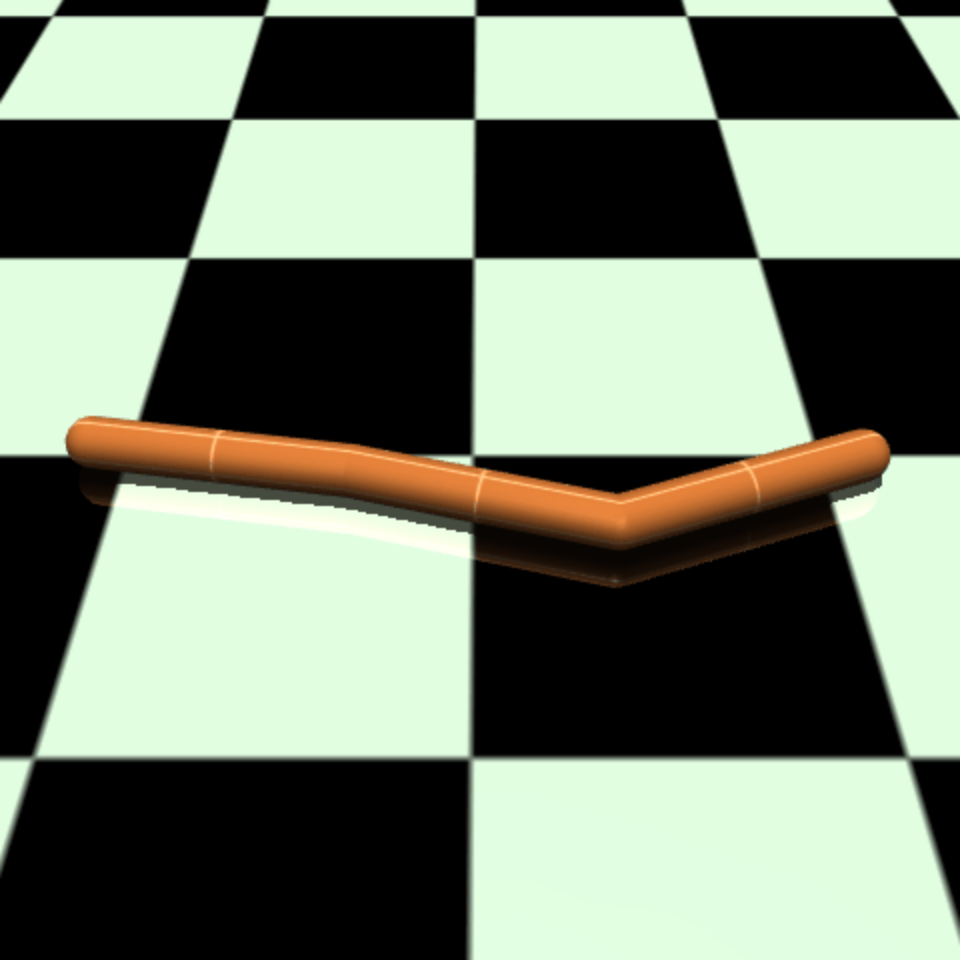
\includegraphics[width=0.18\linewidth]{figs/mujoco_swimmer.png}
    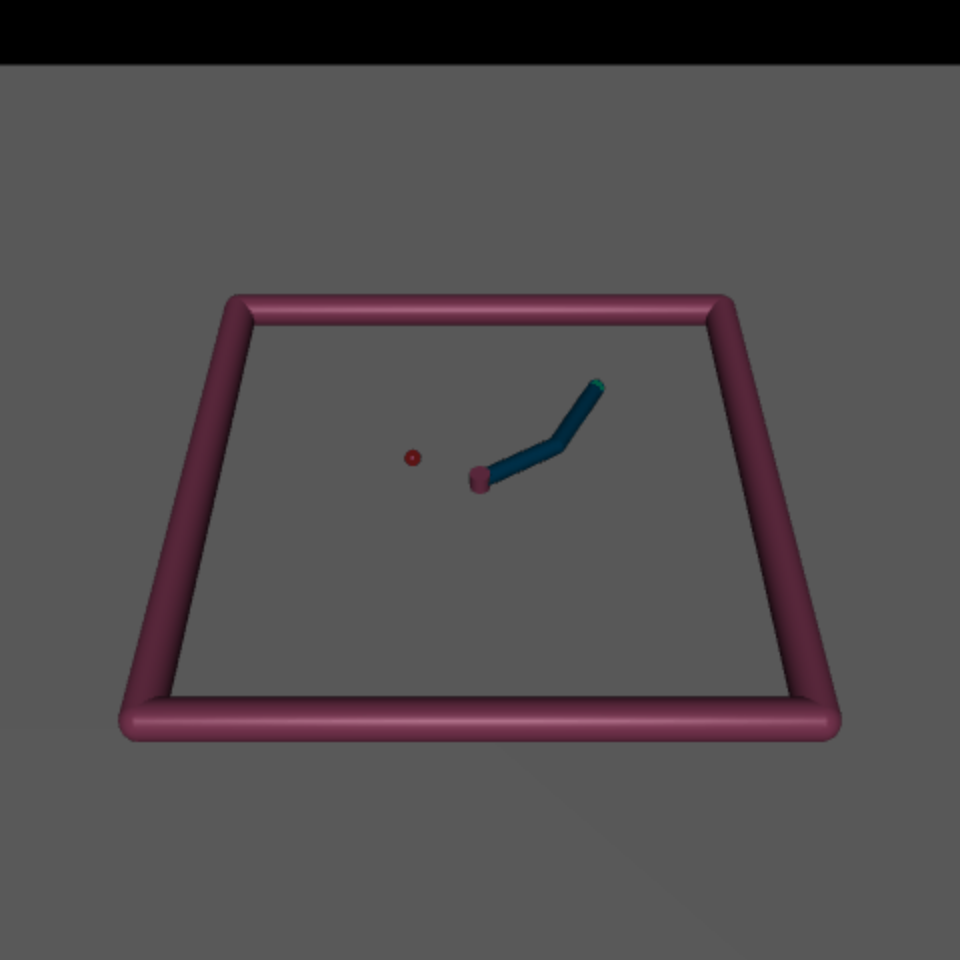
\includegraphics[width=0.18\linewidth]{figs/mujoco_reacher.png}
    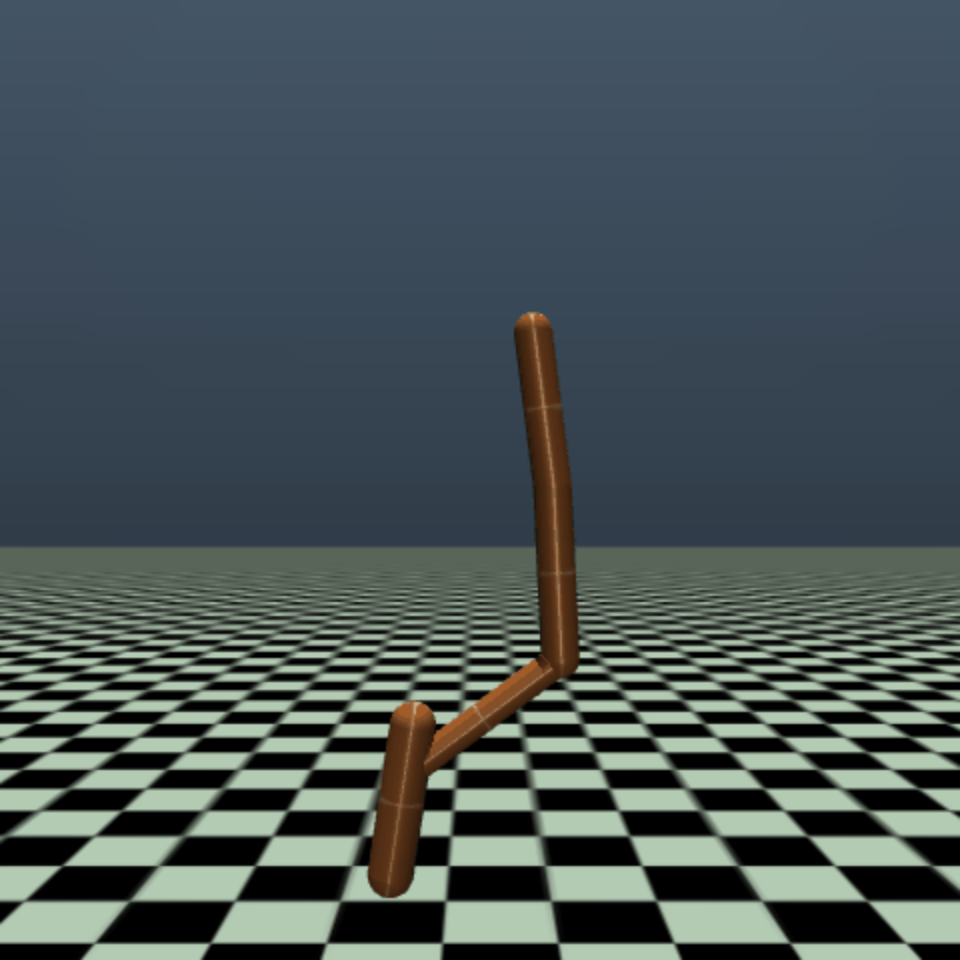
\includegraphics[width=0.18\linewidth]{figs/mujoco_hopper.png}
    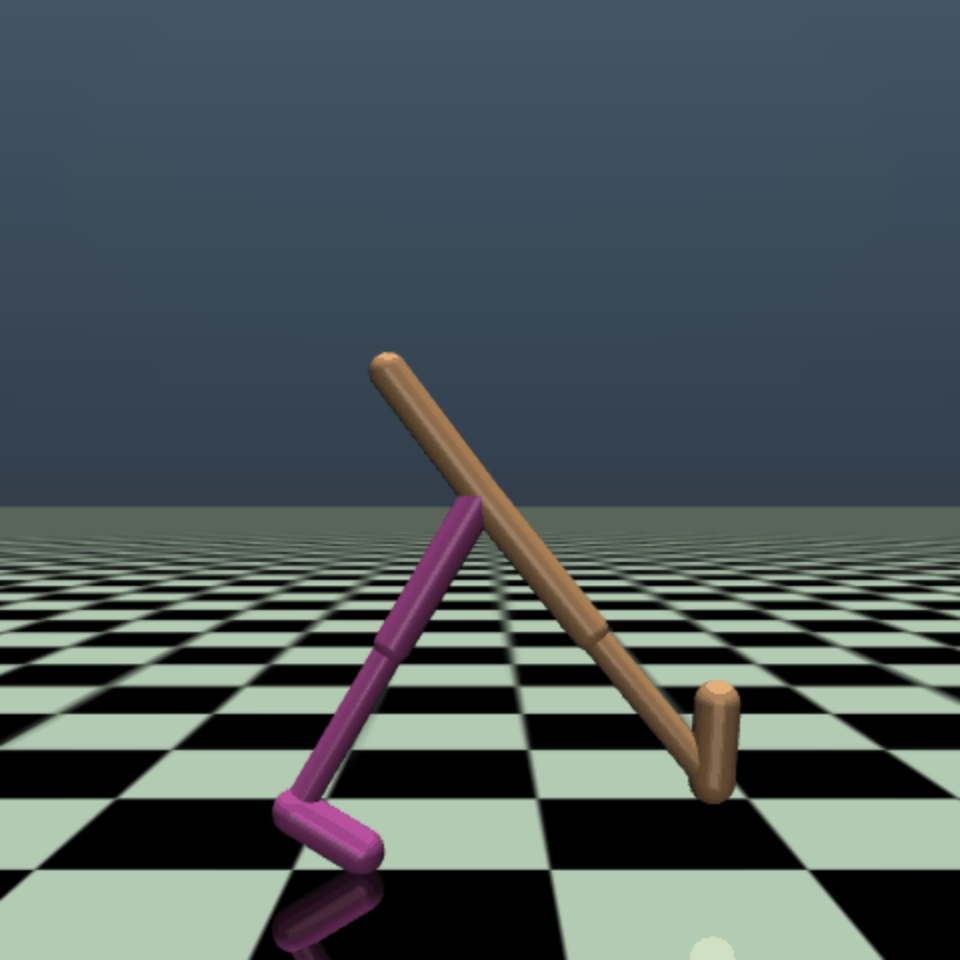
\includegraphics[width=0.18\linewidth]{figs/mujoco_walker.png}
    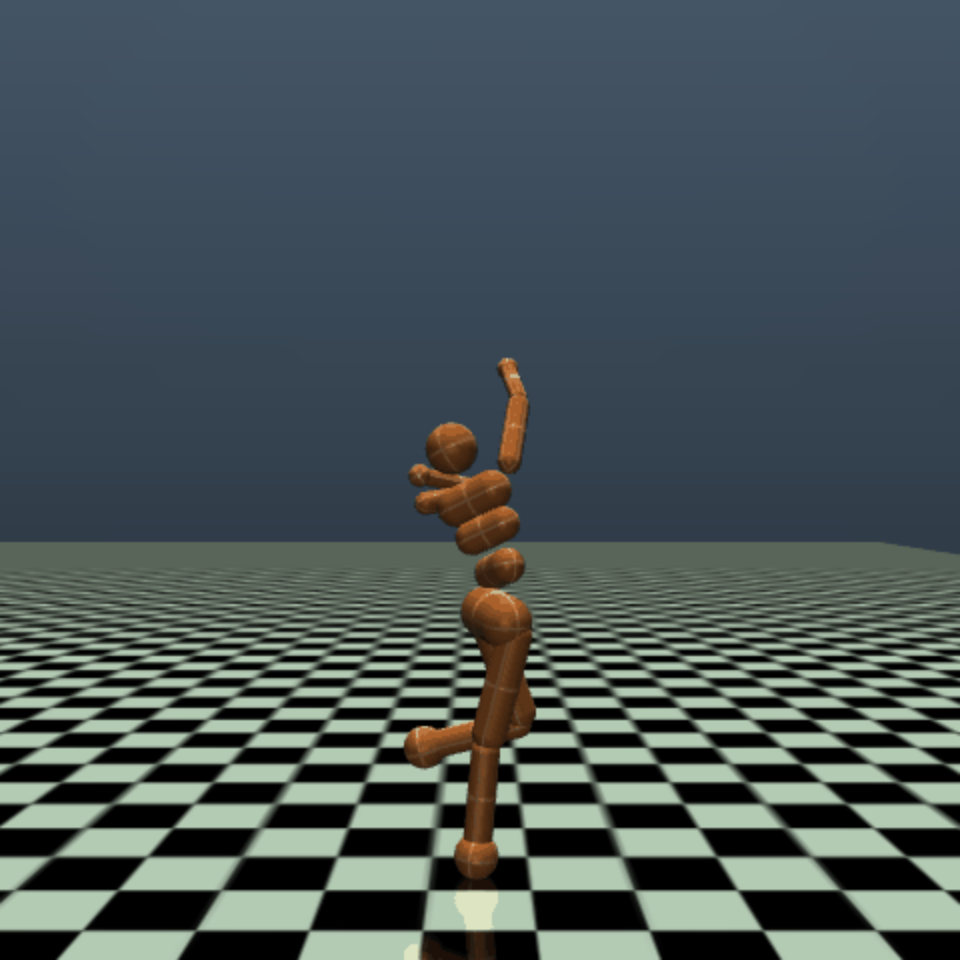
\includegraphics[width=0.18\linewidth]{figs/mujoco_humanoid.png}
    \caption{MuJoCo datasets: \textsc{Swimmer}, \textsc{Reacher}, \textsc{Hopper}, \textsc{Walker2d} and \textsc{Humanoid} environments (left to right).}
    \label{fig:mujoco}
\end{figure}
\begin{table}[]
\footnotesize
\centering
\begin{tabular}{@{}lllllll@{}}
\toprule
                             & BC    & BC-10\% & TD3+BC & AWAC  & CQL   & IQL   \\ \midrule
halfcheetah/simple-v0        & 46.0  & 45.7    & 48.8   & 49.5  & 47.8  & 49.1  \\
halfcheetah/medium-v0        & 95.2  & 94.3    & 87.3   & 95.9  & 88.8  & 93.8  \\
halfcheetah/expert-v0        & 105.6 & 79.5    & 50.0   & 108.5 & 65.2  & 107.1 \\ \midrule
\textit{halfcheetah average} & 82.3  & 73.2    & 62.0   & 84.6  & 67.3  & 83.4  \\ \midrule
hopper/simple-v0             & 83.4  & 83.6    & 83.6   & 83.9  & 82.6  & 83.7  \\
hopper/medium-v0             & 94.5  & 94.7    & 94.5   & 96.4  & 94.0  & 94.7  \\
hopper/expert-v0             & 108.4 & 109.1   & 107.9  & 108.1 & 107.1 & 106.1 \\ \midrule
\textit{hopper average}      & 95.4  & 95.8    & 95.4   & 96.1  & 94.5  & 94.8  \\ \midrule
walker2d/simple-v0           & 61.9  & 62.4    & 63.8   & 62.1  & 62.0  & 64.4  \\
walker2d/medium-v0           & 91.0  & 91.5    & 91.5   & 91.2  & 91.8  & 91.5  \\
walker2d/expert-v0           & 101.9 & 102.1   & 101.4  & 29.4  & 100.3 & 102.3 \\ \midrule
\textit{walker2d average}    & 85.0  & 85.3    & 85.6   & 60.9  & 84.7  & 86.1  \\ \bottomrule
\end{tabular}
\caption{Normalized scores of offline RL algorithms on the MuJoCo locomotion datasets generated in Minari, using the CORL~\cite{corl} implementations. Each cell is the mean over 3 seeds of the best-checkpoint policy (the maximum over evaluation checkpoints during the $10^6$ gradient steps of training), evaluated for 10 episodes; italicised rows give per-environment averages over the three skill tiers. We report the best rather than the final checkpoint because off-policy actor-critic offline methods (notably TD3+BC, AWAC, and CQL) are known to become unstable and diverge at the final checkpoint on narrow expert datasets, so the last-checkpoint score can substantially understate the performance reached during training; reporting both the last and best checkpoint is standard practice in offline RL~\cite{corl}. Scores use the same normalization as Table~\ref{tab:benchmarks_d4rl}, $100\,(R-R_{\min})/(R_{\max}-R_{\min})$, with $R_{\min}$ the mean return of a random policy (50 episodes) and $R_{\max}$ the mean return of the corresponding \textit{expert} dataset. Note that, unlike the canonical D4RL normalization, $R_{\max}$ here is Minari's own expert-dataset mean rather than a fixed reference expert score; because Minari's SAC/TQC experts are stronger than D4RL's reference experts (e.g.\ $1.34\times$ on \textsc{HalfCheetah} and $1.49\times$ on \textsc{Walker2d}), a score of $100$ corresponds to a higher absolute return than in D4RL, and these values are therefore not directly comparable to published D4RL scores.}
\label{tab:benchmarks_mujoco}
\end{table}
We provide comprehensive datasets for all MuJoCo \cite{mujoco} robotic tasks available in the Gymnasium package \cite{andreasthesis}. These datasets were generated using Stable Baselines 3 \cite{sb3}, primarily employing Soft Actor Critic \cite{sac}, with Truncated Quantile Critics \cite{tqc} used specifically for the complex \textsc{Humanoid} environment. By strategically early-stopping training at different performance plateaus, we created multiple dataset variants that capture diverse skill levels. These varied performance levels are important for evaluating algorithm robustness with imperfect datasets, better reflecting real-world applications.

For balancing tasks (\textsc{InvertedPendulum}, \textsc{InvertedDoublePendulum}), we offer expert datasets (perfect balance maintenance) and medium datasets (balance sustained for approximately 100 steps). Arm manipulation environments (\textsc{Reacher}, \textsc{Pusher}) similarly include expert variants (efficient goal achievement) and medium variants (suboptimal but functional performance).
Our 2D locomotion environments (\textsc{HalfCheetah}, \textsc{Hopper}, \textsc{Walker2D}) feature three performance tiers: expert (optimal natural motion), medium (competent but suboptimal movement), and simple (basic functional locomotion). The \textsc{Swimmer} environment includes expert (efficient serpentine motion) and medium (functional but inefficient movement) variants.
For more complex locomotion, \textsc{Ant} datasets span expert (fast galloping with occasional falls), medium (stable rapid walking), and simple (slow, highly stable movement) variants. \textsc{Humanoid} similarly provides expert (running), medium (brisk walking), and simple (slow, sliding movement) variants.

\subsection{BabyAI}
\begin{figure}[t!]
    \centering
    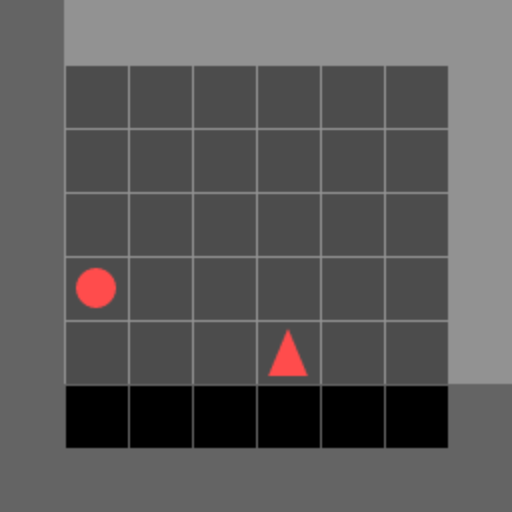
\includegraphics[width=0.18\linewidth]{figs/babyai_gotoredballnodists.png}
    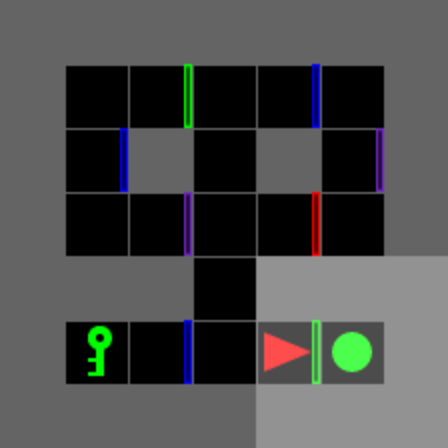
\includegraphics[width=0.18\linewidth]{figs/babyai_keycorridors3r3.png}
    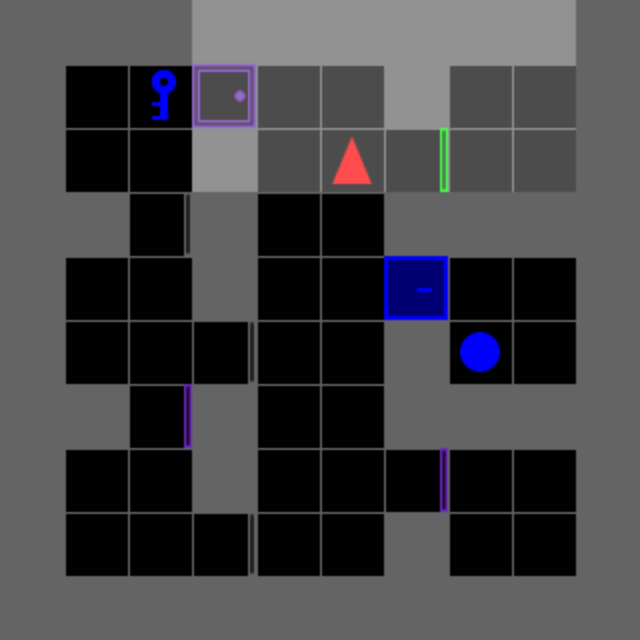
\includegraphics[width=0.18\linewidth]{figs/babyai_keycorridors4r3.png}
    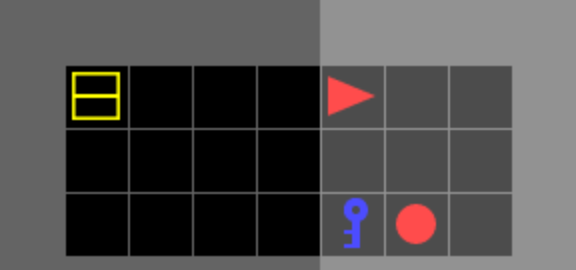
\includegraphics[width=0.384\linewidth]{figs/babyai_movetwoacrosss5n2.png}
    \caption{BabyAI datasets: \textsc{GoToRedBall}, \textsc{KeyCorridor} (two variants), and \textsc{MoveTwoAcross} tasks (left to right).}
    \label{fig:babyai}
\end{figure}
BabyAI \cite{babyai} presents a suite of instruction-following tasks in grid world environments designed to study grounded language learning. These environments feature an agent that must interpret and execute natural language instructions in partially observable grid-based worlds. The tasks range from simple navigation commands to complex multi-step instructions involving object manipulation.

We generated 170 distinct datasets spanning the entire BabyAI task hierarchy, from basic GoToRedBall scenarios to complex instruction following in BossLevel. For each environment, we created two dataset variants: (1) with agent-centric partial observations that simulate a limited field of view, and (2) with full grid observations providing complete state information. This dual representation enables research on both partially observable and fully observable instruction-following tasks.

All trajectories were collected using the deterministic expert policy provided in the BabyAI framework, which generates optimal solutions for each task. Each dataset contains 1,000 complete episodes, ensuring sufficient data for training and evaluation. The datasets capture diverse linguistic instructions paired with the corresponding state-action trajectories required to fulfill them, providing a rich resource for studying language grounding, hierarchical planning, and instruction following in reinforcement learning.


\subsection{Atari}
\begin{figure}[t!]
    \centering
    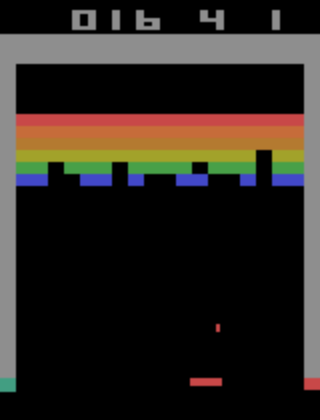
\includegraphics[width=0.18\linewidth]{figs/atari_breakout.png}
    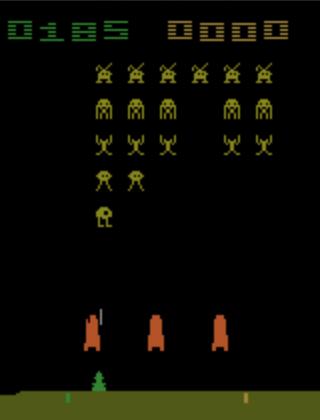
\includegraphics[width=0.18\linewidth]{figs/atari_spaceinvaders.png}
    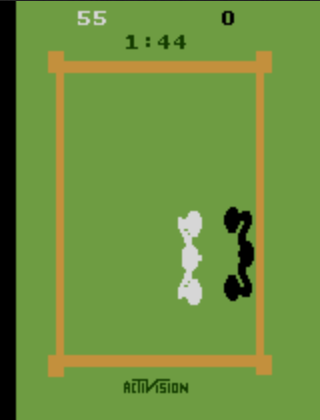
\includegraphics[width=0.18\linewidth]{figs/atari_boxing.png}
    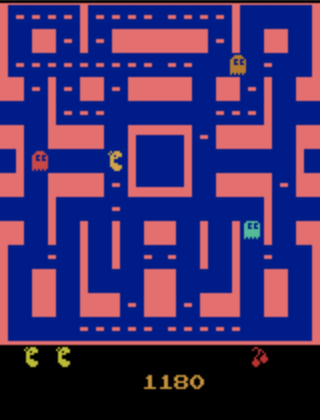
\includegraphics[width=0.18\linewidth]{figs/atari_mspacman.png}
    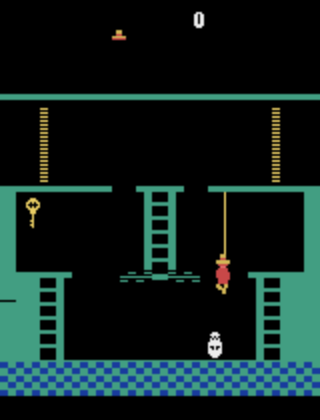
\includegraphics[width=0.18\linewidth]{figs/atari_montezuma.png}
    \caption{ALE datasets: \textsc{Breakout}, \textsc{Space Invaders}, \textsc{Boxing}, \textsc{Ms PacMan} and \textsc{Montezuma's Revenge} environments (left to right).}
    \label{fig:atari}
\end{figure}
The Arcade Learning Environment (ALE) \cite{ALE} serves as a foundational benchmark in reinforcement learning research. We collected expert demonstrations across 57 distinct Atari 2600 games, capturing diverse gameplay dynamics and challenge levels. For each environment, we recorded 10 complete episodes using pretrained agents from CleanRL \cite{cleanrl}, which implemented PPO \cite{ppo} with IMPALA architecture \cite{impala}. While the policy employs standard preprocessing techniques such as frame stacking, grayscale conversion, and resizing, the dataset preserves raw images as observations, allowing users the flexibility to apply their own preprocessing methods.

The collection spans diverse game types including shooting games (Space Invaders), maze navigation (Ms. Pac-Man), sports simulations (Boxing), and puzzle environments (Montezuma's Revenge). These datasets provide several unique characteristics that complement our other collections: pixel-based observations, longer temporal dependencies, diverse reward structures, and established performance benchmarks. This makes them particularly valuable for research in representation learning, credit assignment, and visual policy learning across the spectrum of reinforcement learning challenges.

\subsection{MetaWorld}
MetaWorld \cite{metaworld} provides a benchmark of 50 diverse robotic manipulation tasks designed for multi-task and meta-reinforcement learning research. Each task features a simulated Sawyer robotic arm performing various operations (reaching, pushing, pick-and-place, tool use, door manipulation, and button pressing) within a MuJoCo environment. We generated datasets for all 50 tasks using the deterministic expert policies provided in the official MetaWorld package, collecting 50 complete episodes per task. These policies, built on a heuristic controller, demonstrate near-optimal performance across environments.

The datasets preserve full state information, including the 3D hand position, end-effector configuration, object properties, and goal position. This makes them valuable for various research applications in offline reinforcement learning, transfer learning, and skill composition. Unlike the D4RL manipulation datasets that focus on high-dimensional dexterous manipulation, these datasets emphasize a wider variety of structured tasks with clearly defined success criteria.


\subsection{WebAgents}
We integrated WebLINX \cite{weblinx}, a large-scale dataset of web interactions, into the Minari format. WebLINX contains 24K interactions across 969 successful trajectories of agents completing tasks on the web. This dataset demonstrates Minari's broad applicability beyond traditional reinforcement learning scenarios, as it consists primarily of text-based observations and actions without explicit reward signals.

The trajectories capture diverse web navigation tasks, including form completion, information retrieval, and multi-step workflows across various websites. By supporting this dataset format, Minari enables researchers to readily apply offline reinforcement learning techniques to web automation, text-based agents, and instruction following in browser environments.


\section{Benchmarks}

Minari's primary contribution is infrastructure rather than a new algorithm: its goal is to provide a standard and tooling for RL datasets, while the benchmarking of specific algorithms is best served by the dedicated offline RL libraries that integrate Minari (Sec.~\ref{sec:integrations}). Nevertheless, to demonstrate that our regenerated datasets are usable and yield results consistent with the literature, we report reference scores for the subset of datasets that reproduce the original D4RL benchmark~\cite{d4rl}. We evaluate six widely used offline RL algorithms, BC, BC-10\%, TD3+BC~\cite{TD3+BC}, AWAC, CQL~\cite{CQL}, and IQL, using the implementations and tuned hyperparameters from CORL~\cite{corl}, and report normalized scores in Tables~\ref{tab:benchmarks_d4rl} and~\ref{tab:benchmarks_mujoco}. These results are intended as sanity-check baselines and a starting point for the community, not as an exhaustive evaluation.


% \section{Maintenance, hosting, and accessibility}
% \label{sec:maintenance}
% Minari is developed and maintained by the Farama Foundation, a non-profit organization that stewards widely used reinforcement learning libraries (including Gymnasium and PettingZoo), providing long-term institutional support beyond the lifespan of a single research project. The library is released under the MIT license, is distributed on PyPI, and is developed openly on GitHub, where issues and contributions are reviewed continuously by maintainers and the community. Datasets are versioned and hosted on the HuggingFace Hub, which provides reliable, persistent, and free public access, while the generation scripts are kept in a separate public repository so that every dataset can be regenerated from scratch. Comprehensive documentation, tutorials, and an API reference are available at the project website. Re-packaged third-party datasets (e.g., WebLINX) retain and credit their original licenses, and authorship and licensing information is recorded in each dataset's metadata. This combination of an institutional steward, permissive licensing, open generation scripts, and hosted versioned data is designed to ensure the long-term availability, reproducibility, and extensibility of the collection.

\section{Conclusion}
This paper introduces Minari, an open-source library designed to address the important challenges of standardization, reproducibility, and interoperability in reinforcement learning datasets. By establishing a unified framework for collecting, manipulating, and sharing agent experience data, Minari significantly lowers the barriers to collaboration and accelerates progress in offline reinforcement learning research.

The library's feature set supports the entire dataset lifecycle, from initial collection to sharing and reuse. Its adherence to consistent naming conventions, detailed metadata, and flexible file formats ensures that datasets are both accessible and reproducible. The seamless integration with major offline reinforcement learning frameworks like TorchRL, AgileRL, and D3RLPY further enhances its utility within existing research workflows.

Our curated collection of \numdatasets datasets spanning robotics, navigation, instruction following, Atari games, and web interactions provides a concrete resource for the research community, with \numtrajectories unique trajectories totaling \numsteps interaction steps. This diverse collection enables researchers to benchmark algorithms across multiple domains and complexity levels without the overhead of dataset generation and processing.

Despite these advantages, Minari has certain limitations. Since data is saved in episodes and read as batches of episodes, Minari may struggle with life-long episodes in open-ended tasks where clear episode boundaries are not defined. Additionally, while Minari relies on high-efficiency data formats, it might introduce overhead compared to highly-optimized training pipelines with specialized data loaders.

As we continue to expand Minari's capabilities and dataset collection, we envision it becoming a major infrastructure for advancing data-driven reinforcement learning. By standardizing the way agent experience is shared and reused, Minari aims to foster a more collaborative research ecosystem where insights and innovations can build upon each other more efficiently.
https://github.com/kourgeorge/arxiv-style
\section*{Acknowledgments}
We acknowledge every contributor, please find the complete list here: \url{https://github.com/Farama-Foundation/Minari/graphs/contributors}

\bibliographystyle{plainnat}
\bibliography{refs}


%%%%%%%%%%%%%%%%%%%%%%%%%%%%%%%%%%%%%%%%%%%%%%%%%%%%%%%%%%%%

\appendix


\section{Dataset Metadata}

Both datasets and individual episodes can have metadata attached to them. The dataset metadata can be specified by the user during dataset creation. When creating a Minari dataset the default global metadata will be the ones reported in Table \ref{tab:metadata}.

\begin{table}[H]
    \centering
    \begin{tabular}{lll}
    \toprule
        Attribute & Type & Description \\ \midrule
        \pythoninline{dataset_id} & \pythoninline{str} & Identifier of the Minari dataset. \\
        \pythoninline{total_episodes} & \pythoninline{int} & Number of episodes in the Minari dataset. \\
        \pythoninline{total_steps} & \pythoninline{int} & Number of steps in the Minari dataset. \\
        \pythoninline{action_space} & \pythoninline{Space} & Gymnasium action space describing actions in dataset. \\
        \pythoninline{observation_space} & \pythoninline{Space} & Gymnasium observation space describing observations in dataset. \\
        \pythoninline{env_spec} & \pythoninline{str} & JSON string of the Gymnasium environment spec. \\
        \pythoninline{code_permalink} & \pythoninline{str} & Link to a repository with the code used to generate the dataset. \\
        \pythoninline{author} & \pythoninline{set of str} & Name of the authors that created the dataset. \\
        \pythoninline{author_email} & \pythoninline{set of str} & Email of the authors that created the dataset. \\
        \pythoninline{algorithm_name} & \pythoninline{str} & Name of the expert policy used to create the dataset. \\
        \pythoninline{minari_version} & \pythoninline{str} & Version of Minari that generated the dataset. \\
        \pythoninline{requirements} & \pythoninline{list of str} & List of requirements in pip-style to load the environment. \\ \bottomrule
    \end{tabular}
    \caption{List of metadata attributes of a Minari dataset.}
    \label{tab:metadata}
\end{table}

Only \pythoninline{dataset_id}, \pythoninline{total_episodes}, and \pythoninline{total_steps} are mandatory (with the latter two automatically computed). Metadata for each episode is also supported and can be added by the user via a callback function. The episode statistics for the observed rewards are automatically computed.

\section{Environment support}

The Minari storage format supports the following observation and action spaces:

\begin{table}[H]
    \centering
    \begin{tabular}{lll}
        \toprule
        Space & Description & \\ \midrule
        \pythoninline{Box} & An n-dimensional continuous space. & \\
        \pythoninline{Discrete} & Describes a discrete space with an observation in $\{0, 1, ..., n-1\}$. & \\
        \pythoninline{MultiDiscrete} & Represents the cartesian product of arbitrary Discrete spaces. & \\
        \pythoninline{MultiBinary} & A binary space. The elements are binary arrays. & \\
        \pythoninline{Tuple} & Represents a tuple of spaces. & \\
        \pythoninline{Dict} & Represents a dictionary of spaces. & \\
        \pythoninline{Text} & The elements of this space are bounded strings from a charset. & \\ \bottomrule
    \end{tabular}
\end{table}

\section{Episode data structure}

A Minari dataset is encapsulated in the `MinariDataset` class which allows for iterating and sampling through episodes which are defined as \pythoninline{EpisodeData} data class. Take the following example where we load the \pythoninline{D4RL/door/human-v2} dataset and randomly sample 10 episodes:

\begin{python}
import minari
dataset = minari.load_dataset("D4RL/door/human-v2", download=True)
sampled_episodes = dataset.sample_episodes(10)
\end{python}

The \pythoninline{sampled_episodes} variable will be a list of 10 \pythoninline{EpisodeData} elements, each containing episode data. An \pythoninline{EpisodeData} element is a data class consisting of the following fields:

\begin{table}[H]
    \centering
    \begin{tabular}{lll}
    \toprule
        Field & Type & Description \\ \midrule
        \pythoninline{id} & \pythoninline{int} & ID of the episode. \\
        \pythoninline{observations} & \pythoninline{np.ndarray}, \pythoninline{list}, \pythoninline{tuple}, \pythoninline{dict} & Stacked observations for each step. \\
        \pythoninline{actions} & \pythoninline{np.ndarray}, \pythoninline{list}, \pythoninline{tuple}, \pythoninline{dict} & Stacked actions for each step. \\
        \pythoninline{rewards} & \pythoninline{np.ndarray} & Rewards for each step. \\
        \pythoninline{terminations} & \pythoninline{np.ndarray} & Terminations for each step. \\
        \pythoninline{truncations} & \pythoninline{np.ndarray} & Truncations for each step. \\
        \pythoninline{infos} & \pythoninline{dict} & Additional information returned by the environment \\ \bottomrule
    \end{tabular}
\end{table}

where the specific type of the observation and action depends on their respective spaces.


\end{document}
